\section{Rocket Attitude Module}

\subsection{Rocket Attitude Display Module}
The Rocket Attitude display takes in IMU data and a 3D model. It renders this 3D model, and then 
uses IMU data from the rocket to alter the orientation of the model to match that of the live rocket.

\subsubsection{Model Storage}
There is an offline storage which stores the 3D model, as well as the material that is applied to the model.

\subsection{IMU Data Calculations}
The system performs any necessary computations on the IMU data to make it usable for the display module.

\subsubsection{Smoothing Calculations}
The default rotating of the rocket model sometimes causes choppy animation. As a result, the rotating
goes through a smoothing process in order to ensure a smooth display.

\subsection{Display Output}
The module uses a rendered 3D model, along with the processed and smoothed data, to produce a live 
simulation of the real rocket's attitude during its flight.

\begin{figure}[ht!]
\centering
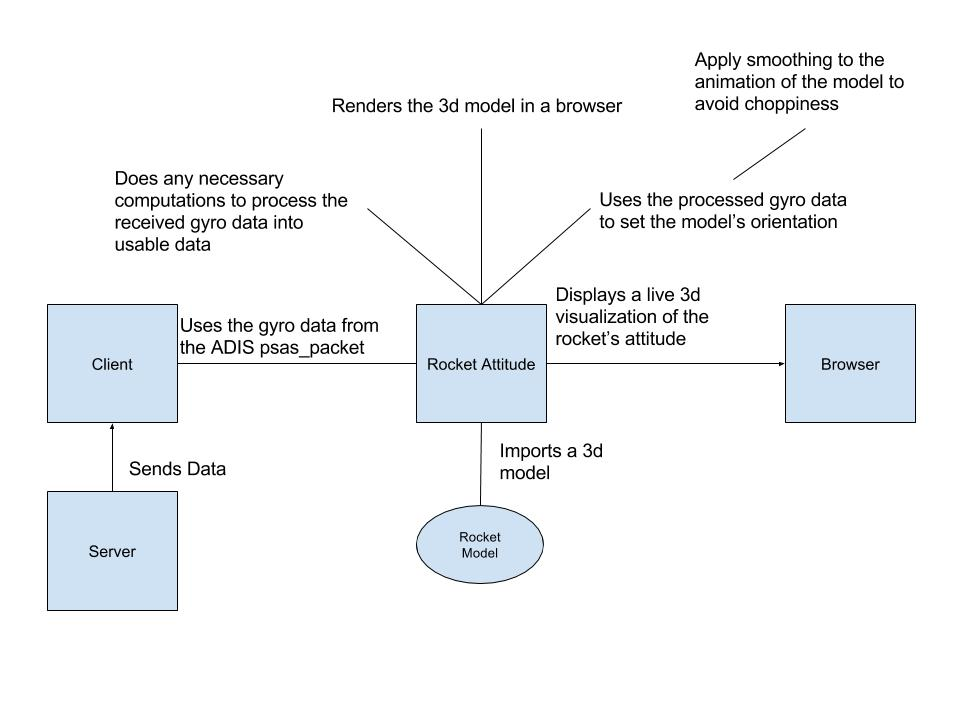
\includegraphics[scale=.4]{imgs/attitude.jpg}
\caption{Rocket Attitude \label{overflow}}
\end{figure}
